% !TEX root = ./../../_Thesis.tex

% section's Name and Label
\section{Sensation and Perception}
\label{sec:SensationAndPerception}

Sensation and perception are the processes that put us in contact with stimuli from our world --- objects and events \cite{King2012}. Understanding these processes requires comprehending the physical properties of our perception and the study of the corresponding sensor,
%sense organ, 
for example, light and the eye. \citet{Lemma2005} defines some concepts that are necessary to explain how stimulation (\eg, visual information) becomes meaningful perception: (i) {\it stimulus}: a source of physical energy that produces a response in a sense organ; (ii) {\it response}: any reaction of an organism to or in the presence of a stimulus; (iii) {\it transduction}: sequence of operations by which physical energy is transformed into patterns of neural impulses that give rise to sensory experience; (iv) {\it sensation}: process of receiving stimulus energies from external environment and transforming those energies into neural energy; and (v) {\it perception}: process whereby the brain interprets sensations, taking into account past experiences, the context in which the sensation occurs, and emotions.

The steps related to the perception of a visual information are illustrated in Figure \ref{fig:flow}, where light waves reflected from the butterfly act as stimuli to react with our sensory receptors, which convert the energy into neural signals. After that, neural messages travel to the sensory cortex of the brain and become sensations. Finally, the process of perception interprets these sensations and grant us to recognize a butterfly \cite{Zimbardo2012}.

\begin{figure}[h]
	\centering
	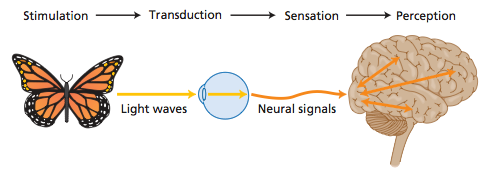
\includegraphics[width=0.73\linewidth]{__Images/02/flow.png}
	\caption[General flow of sensory information]{General flow of sensory information from energy stimulus to sensory receptor cell to sensory neuron to sensation and perception \cite{Zimbardo2012}.}
	\label{fig:flow}
\end{figure}

Light is a form of electromagnetic (EM) radiation which travels through space in waves and can be described in terms of its physical characteristics --- wavelengths and/or amplitude. Color and brightness are the psychological counterparts of light wavelength and intensity that exist only in the brain \cite{King2012}. Humans are capable of detecting only a tiny segment of the EM spectrum, called visible light (Figure \ref{fig:spectrum}), which ranges in wavelength from approximately 400 to 700 nm (1nm = 10$^{-9}$m). 
Wavelengths outside this range are not detected by humans because they are not transmitted by the ocular media or cannot be absorbed by our retinal photopigments \citet{Schwartz2010}.
%Schwartz \citet{Schwartz2010} "other wavelengths are not visible, either because the ocular media does not transmit them or because they are not absorbed by the retinal photopigments".

\begin{figure}[h]
	\centering
	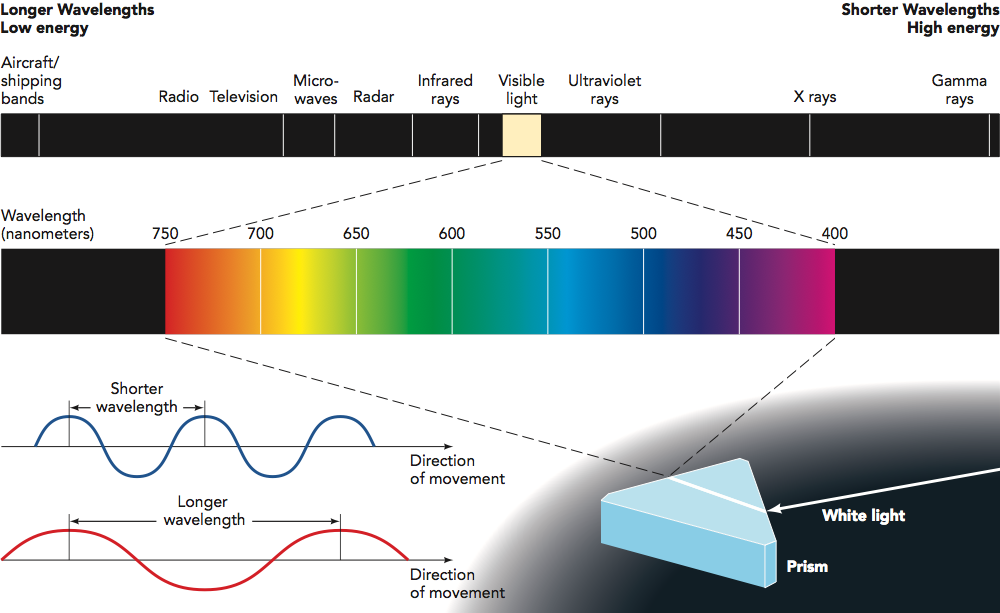
\includegraphics[width=0.95\linewidth]{__Images/02/spectrum.png}
	\caption[The Electromagnetic Spectrum and Visible Light]{The Electromagnetic Spectrum and Visible Light: (Top) Visible light is only a narrow band in the electromagnetic spectrum. Visible light wavelengths range from 400 to 700 nanometers. X rays are much shorter, radio waves much longer. (Bottom) The two graphs show how waves vary in length between successive peaks. Shorter wavelengths are higher in frequency, as reflected in blue colors; longer wavelengths are lower in frequency, as reflected in red colors \cite{King2012}.}
	\label{fig:spectrum}
\end{figure}


%\begin{quote}
%All sensations begins with sensory receptors. Sensory receptors are specialized cells that detect stimulus information and transmit it to sensory nerves and the brain [...] creating local electrical currents. These currents are graded; that means they are sensitive to the intensity of stimulation, such as the difference between a dim and a bright light \cite[p. 80]{King2012}.  
%\end{quote} 
%%\

Distinct neural messages flows into the nervous system as information, and it's type depends on the energy captured by a sensory receptor. Figure \ref{fig:senses} shows the human sensory receptors for vision, hearing, touch, smell, and taste. In order to generate a sensory experience from any receptor, there is a minimal amount of physical energy needed - known as absolute threshold \cite{Zimbardo2012}.

\begin{figure}[h]
	\centering
	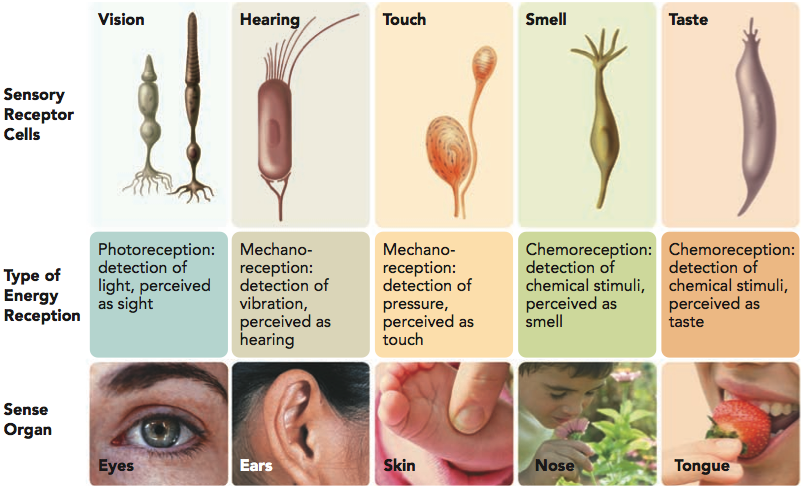
\includegraphics[width=0.95\linewidth]{__Images/02/senses.png}
	\caption[Human Senses: organs, energy stimuli, and sensory receptors]{Human Senses: organs, energy stimuli, and sensory receptors \cite{King2012}.}
	\label{fig:senses}
\end{figure}

Table \ref{table:threshold} shows some typical absolute threshold levels for several familiar stimuli. Experiments designed to determine thresholds, and the study of the relationship between physical nature of stimuli and people's response to them belong to a branch of psychology called {\it psychophysics} \cite{Lemma2005}.

\begin{table}[h]
	\caption[Sensory threshold of five senses]{Sensory threshold of five senses \cite{Zimbardo2012}.}
	\begin{center}
	\begin{tabular}{l l}
	
		\textbf{Sense}	&	\textbf{Detection Threshold} \\
		\hline
		Sight			&	A candle flame at 30 miles on a clear, dark night\\
		Hearing			&	The tick of a watch 20 feet away in a quiet room\\
		Smell			&	One drop of perfume diffused throughout a three-room apartment\\
		Taste			&	One teaspoon of sugar in 2 gallons of water\\
		Touch			&	A bee's wing falling on the cheek from 1 centimeter above\\
	\end{tabular}
	\end{center}
	\label{table:threshold}
\end{table}

%According to \citet{Blake2005}, "understanding perception also makes it possible to design devices to help individuals with impaired sensory function". The following sections focus on aspects of sensation and perception concerning the visual system, and details psychophysical methods for studying perception that could be used to improve individual's visual experience.